%
% File: chap01.tex
%
\let\textcircled=\pgftextcircled
\chapter{Theory}
\label{chap:intro}

\initial{A} neutron poison is an element that absorbs neutrons of interest in a nuclear reactor core. In most reactors today, the neutrons of interest are the thermal neutrons, with low energies. Those are the neutrons driving the chain reaction, by fissioning the $^{235}U$. Different types of neutron poisons can be identified, the design absorbers and the fission products absorbers. One of the most potent neutron absorber known is the Xenon, the fission product subject of this project. The impact of Xenon on a nuclear reactor was discovered in 1944 in the USA, when a reactor experienced strange behavior in its power buildup. Xenon is not the only poison of interest in a nuclear reactor. Indeed, Samarium is also to be taken into account, though in a much lesser way. The presence of Samarium ($^{149}Sm$) in a classical pressurized water reactor will not prohibit it from operating normally like Xenon can. However, it will impact the rod calibration if not accounted for while predicting the measurements.

One can note that in order to ease the reading, the terms Xenon and Iodine will be used interchangably with the terms $^{135}Xe$ and $^{135}I$. The theory is based on the course handouts~\cite{reactor01}, as well as various Nuclear Reactor Physics books.



\section{Fission products}

The fission of an atom caused by a neutron create a number of neutrons and new atoms, fission products. Only a few of the fission products are responsible for most of their effects, the decay heat and additional neutron absorption. The most potent product fission absorber is the Xenon 135 ($^{135}Xe$). Another noteworthy fission product is the Samarium 149 ($^{149}Sm$).

\begin{figure}[t!]
	\centering
	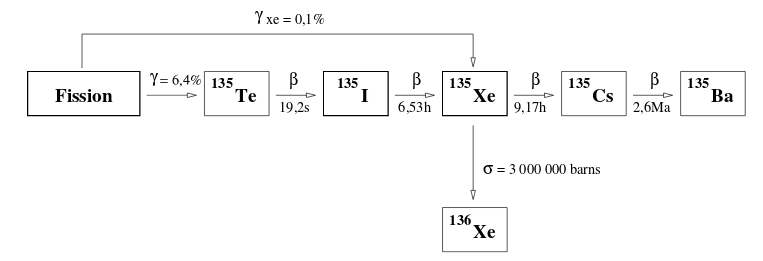
\includegraphics[height=0.2\textheight]{fig01/xenon_chain.png}
	\mycaption[Creation process of $^{135}Xe$]{Creation process of $^{135}Xe$.}
	\label{fig:chain}
\end{figure}

\begin{figure}[t!]
	\centering
	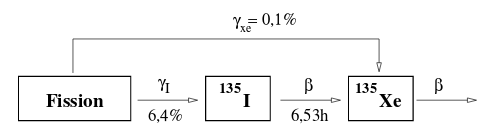
\includegraphics[height=0.1\textheight]{fig01/xenon_chain_simp.png}
	\mycaption[Simplified creation process of $^{135}Xe$]{Simplified creation process of $^{135}Xe$.}
	\label{fig:chain_simp}
\end{figure}

Figure~\ref{fig:chain} presents the most common $^{135}Xe$ creation process in a nuclear reactor. Due to the short half-life of the Tellurium 135, it can be neglected, and the process will be simplified to the one presented in figure~\ref{fig:chain_simp}.

We can describe this simplified process mathematically:

\begin{equation}
\frac{dC_I}{dt} = \gamma_I \Sigma_f\phi - \lambda_I C_I
\end{equation}

\begin{conditions}
 C_I   &  Population of $^{135}I$ per $cm^{3}$ \\
 \gamma_I   &  Fission product yield of $^{135}I$ \\
 \Sigma_f   &  Macroscopic fission section \\
 \phi       & Neutronic flux in $cm^{-2}.s^{-1}$ \\
 \lambda_I  & Radioactive decay constant of $^{135}I$ in $s^{-1}$
\end{conditions}



\begin{equation}
\frac{dC_{Xe}}{dt} = \gamma_{Xe} \Sigma_f\phi + \lambda_I C_I - (\lambda_{Xe} + \sigma_{Xe}\phi) C_{Xe}
\end{equation}

\begin{conditions}
 C_{Xe}   &  Population of $^{135}I$ per $cm^{3}$ \\
 \gamma_{Xe}   &  Fission product yield of $^{135}I$ \\
 \Sigma_f   &  Macroscopic fission section \\
 \sigma_{Xe}   &  Microscopic absorption section \\
 \phi       & Neutronic flux in $cm^{-2}.s^{-1}$ \\
 \lambda_{Xe}  & Radioactive decay constant of $^{135}I$ in $s^{-1}$
\end{conditions}


$^{135}I$ can be produced by the fission of $^{235}U$ with a yield $\gamma_I$, hence a production of $\gamma_I\Sigma_f\phi$ atoms of $^{135}I$, and it can disappear by decay, $\lambda_I C_I$. On the other hand, $^{135}Xe$ can be created by the fission of $^{235}U$ with a yield $\gamma_{Xe}$, and by decay of $^{135}I$, hence a production of $\gamma_{Xe}\Sigma_f\phi + \lambda_I C_I$ atoms of $^{135}Xe$. It can disappear by radioactive decay and by capturing neutrons, thus a disappearance of $\lambda_{Xe} C_{Xe} + \sigma_{Xe}\phi C_{Xe}$.


Similarly, we would be able to compute the population of $^{149}Sm$, given by the decay of the fission product neodymium to prometheum. Prometheum 149 has a half-life of around 53 hours and Samarium 149 is stable. This means that the Samarium starts habing an impact after the core has been shut down for approximately two weeks. Thus, after a reloading operation at a nuclear reactor, the presence of the samarium must be taken into account when computing the reactivity of the core.

Other fission products can act as neutron poisons, though nowhere near as problematic as Xenon or Samarium. However, lumped together, their impact is to take into account. In nuclear power reactor, those are often considered within the scope of the ageing (out-of-flux) of the fuel elements, building up the fission products concentration. They will not prevent the reactor from diverging, but they can modify the peak factor in the reactor and needs to be taken into account when designing the core, especially during the power ramp at startup.

Those poisoning fission products, Xenon, Samarium and various others, are of concern in thermal flux reactor. The Xenon cross-section for fast neutrons, for example, is negligible. In hard spectrum reactors, other poisons can be used.

\section{Other neutron poisons}

Poisons are naturally used in a reactor core design, in the fuel elements directly or in the control rods. Their goal is to allow for the control of the reactor or to modify the neutron flux locally, for example to limit the fluence received by the reactor vessel. The most common design absorbers are the Hafnium, boron carbide (B4C), and AgInCd (AIC, Silver, Indium, Cadmium).


\section{Impact of neutron poisons}

As seen previously, the Xenon has the most impact on the reactor. In the following analysis, this element will be the one looked at. The impact of Xenon poisoning in the core is two-fold. It can prevent the reactor startup, by introducing enough negative reactivity that the critical state cannot be reached, and it can oscillate in the core due to some asymmetry, causing potential local power peaks.

\subsection{Negative reactivity}

$^{135}Xe$ is one of the most efficient thermal neutron absorbers known, with a cross-section (whcih can be seen as of probability of interacting with neutrons) of approximately 3 millions barns for such low-energies neutrons, compared to 550 barns for the $^{235}U$. This means that neutrons are way more likely to interact with the Xenon than with Uranium, hence potentially shutting down the reactor by preventing the chain reaction.

This effect is especially seen during the Xenon peak, within eight hours of the reactor shutdown. Then the Xenon concentration is at its maximum, building upon its equilibrium population from the iodine decay. Luckily, $^{135}Xe$ is not stable, and decays away at a higher rate than the iodine decay buildup.

In effect, this implies that a power reactor has a short window after a shutdown to be able to start up again, before the Xenon peak prevent that. After that time, the operator must wait approximately two days, for the Xenon to decay (half-life of around 9 hours), to start up again. One solution is to shut down progressively. This allows the equilibrium population of iodine and xenon, dependent on the flux, to get low enough that the Xenon peak will not add enough negative reactivity to prevent the following start up.

A minimum Xenon concentration must be considered when computing the reactivity insertion potential of a reactor, to be conservative. Indeed, if the limits are based on a maximum Xenon concentration, once the Xenon peak is passed, the reactivity increases back to nominal levels and can damage the core.

\subsection{Xenon oscillation}

The negative reactivity insertion is troublesome from an operation point of view. One issue that is more important to the reactor safety is the xenon oscillation in the core. This can indeed cause a local power peak, translating to higher temperature and potential fuel damage.

The oscillation is initially caused by a dissymetry in the system, often due to control rods positioning and relative worth, but also due to fuel loading patterns. This dissymetry causes a higher flux in a region of the core, and a lower flux in its symmetric region. A higher flux, as seen in the previous concentration equations, implies that the Xenon will absorb more neutrons, and thus disappear, causing the flux to actually increase. On the other hand, when the flux is lower, the Xenon actually continues to build up from Iodine decay, subsequently lowering the flux even more. Consequently, Iodine concentrations increases with high flux and decreases with low flux. Eventually, this Iodine buildup will reverse the effect, creating the oscillation.

The danger come from the high flux part of the oscillation, where, locally, the power can increase a lot and potentially damage (high temperature) the fuel assemblies. This effect must thus be considered when obtaining the limits on the insertion of reactivity.

\section{Xenon reactivity calculation}

The Xenon-free excess reactivity ($\rho_e$) and the rod control calibration curves are given for the GSTR.

\begin{equation}
\rho_e = 3.44\$
\end{equation}


\begin{equation}
\begin{aligned}
\rho_{transient} = 9.332139E-15 * p^5 - 2.001355E-11 * p^4 + 8.071354E-9*p^3\\
 + 4.851361E-6*p^2 + 5.73739E-5*p\\
\rho_{shim1} = 1.9124E-12 * p^4 - 7.5364E-9 * p^3 + 7.2250E-6 * p^2\\
 + 4.3259E-4 * p\\
\rho_{shim2} = 2.112741E-12*p^4 - 7.624993E-9*p^3 + 7.107704E-6*p^2\\
 + 2.741928E-4*p\\
\rho_{regulation} = 1.83246E-12*p^4 - 1.017529E-8*p^3 + 1.174461E-5*p^2\\
 - 3.147143E-4*p
\end{aligned}
\end{equation}

The total rods worth can thus be computed, based on the real up position in the GSTR:

\begin{equation}
\begin{aligned}
\rho_{transient} = 2.296\$ \\
\rho_{shim1} = 2.034\$ \\
\rho_{shim2} = 1.80\$ \\
\rho_{regulation} = 3.088\$
\end{aligned}
\end{equation}

The Xenon-free reactivity needed to reach criticality is hence given by:

\begin{equation}
\sum_i{\rho_i} - \rho_e
\end{equation}
\begin{conditions}
 i  &  [transient, shim1, shim2, regulation]
\end{conditions}

This works for a criticality achieved at 5W, where the value $\rho_e$ is given. In order to compute the Xenon-free reactivity needed to reach criticality, one can assume that over a small period of time, say 20 minutes, the Xenon concentration remains unchanged. That can be considered true given the $^{135}I$ half-life of approximately 6 hours. Thus, from a critical state at 5W, the power can be increased to nominal value and the reactivity difference can be considered Xenon-free.

\section{Procedure}

Given the timeframe of $^{135}I$ and $^{135}Xe$ concentration changes, with half-lives between 6 and 10 hours, this lab should take several days. The reactor is thus run at full power for 8 hours, shut down, and turned back on the following morning. The position of the rods are noted at various intervals, at constant power. Those position, using the control rods calibration curves, relates to a certain amount of reactivity.

Thus, one can obtain the Xenon reactivity in the core as a function of time, to obtain the Xenon transient.


